\documentclass[10pt,letterpaper]{article}
\usepackage{multicol}
\usepackage{amsmath}
\usepackage{graphicx} 
\usepackage{hyperref}
\usepackage{natbib}
\begin{document}
\title{Determining the Half-Life of the Ortho Positronium via Scintillator and Sodium-22 Beta Decay}


\author{
 Akhil Deshpande \\*
  \\*
 PHY 353L Modern Laboratory \\*
 Department of Physics \\*
 The University of Texas at Austin \\*
 Austin, TX 78712, USA
}
\date{\today}

\maketitle

\begin{abstract}
   In this lab, we used scintillators and an Na-22 source to generate ortho-positronium states. We then analyzed the 
   gamma rays that resulted from the decay of the ortho positronium to determine the half life of an ortho positronium in a 
   Nitrogen filled tube was 108.4 $\pm$ 7.7 ns.
\end{abstract}

\section{Introduction}
A positronium is a bound state of a positron($\text{e}^+$) and an electron($\text{e}^-$). \cite{Zute:2018}
A special property of the positronium is the existence of such a bound state without the comparatively massive
nucleus interacting with either particle. These properties of the positronium allow us to get a clearer understanding
of Quantum Electrodynamics (QED).

The story of its discovery begins with the theoretical predictions of 
Paul Dirac in 1928. Dirac's equation, which 
merged quantum mechanics with special relativity, 
implied the existence of a positively charged electron, 
known as the positron. 
The experimental confirmation of the positron came in 1932 by 
Carl D. Anderson, a discovery that earned him the Nobel Prize in 
Physics and paved the way for the acceptance of antimatter in physics.

The exploration into the interactions between electrons and positrons 
led to the theoretical prediction of positronium by 
John Archibald Wheeler in 1946. Wheeler, known for his work in 
quantum mechanics and later in general relativity, postulated that 
an electron and a positron could form a bound state due to their mutual 
electromagnetic attraction, 
similar to the hydrogen atom but with the notable 
difference that both constituents were of equal mass but opposite charge. 
This prediction was a significant leap, suggesting a unique system 
where matter and antimatter coexisted transiently.

The experimental discovery of positronium followed shortly, confirmed by Martin Deutsch at MIT in 1951. Deutsch's experiments demonstrated the existence of two distinct states of positronium: ortho-positronium, with parallel spins of the electron and positron, and para-positronium, with antiparallel spins. This discovery provided an invaluable laboratory for testing quantum electrodynamics (QED), the theory describing how light and matter interact \cite{Yuly:1999}.

Positronium's properties, particularly its distinct annihilation lifetimes, offered a unique avenue for testing the fundamental principles of QED. The para-positronium decays faster, emitting two gamma photons, whereas ortho-positronium, due to spin conservation rules, decays into three photons and has a longer lifetime. These characteristics were in line with the theoretical predictions of QED, thereby providing a robust test for the theory.
\section{Theoretical Background}
\subsection{Positronium Emission Decay}
When the Sodium-22 isotope decays, it undergoes positronium emission decay. This specific type of decay results in 
the formation of a positronium, through the decay of a proton into a neutron. Sodium-22 decays into an excited state 
of Neon-22, a positron, and a neutrino \cite{Zute:2018}. This type of decay is explained in Fig. 1. As we can see in the figure,
about 91\% of the time, Sodium-22 decays into an excited state of Neon-22. When Neon reverts to a non-excited state, gamma rays 
are expelled. These gamma rays are what we use to determine the counts of positroniums formed during the experiment.
\begin{figure}[ht]
    \begin{center}
        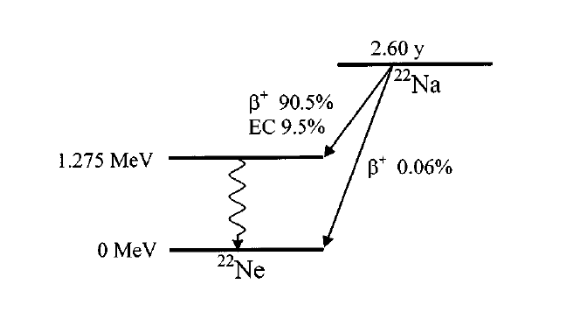
\includegraphics[width=4.5in]{decay.png}
        \caption{Positronium emission decay diagram of Sodium-22, taken from Zute, Campbell 2018}
    \end{center}
\end{figure}

\subsection{Positronium Decay}
As positroniums decay randomly, we can demonstrate their decay function as a differential equation as a function
of time: $$\frac{-dN}{dt} = \lambda N(t)$$
Solving for our elementary variables, we can further simplify:
$$N(t) = N_0e^{-\lambda t}$$
Furthermore, the half life of the positronium ($t_{1/2}$) can be modeled as: $$e^{-\lambda t_{1/2}} = \frac{1}{2}$$
This equation comes from the trivial observation that $t_{1/2}$ occurs when the number of positroniums reaches one half of its original value.
\section{Experimental Setup}
\subsection{Apparatus}
\begin{figure}[!htbp]
    \begin{center}
        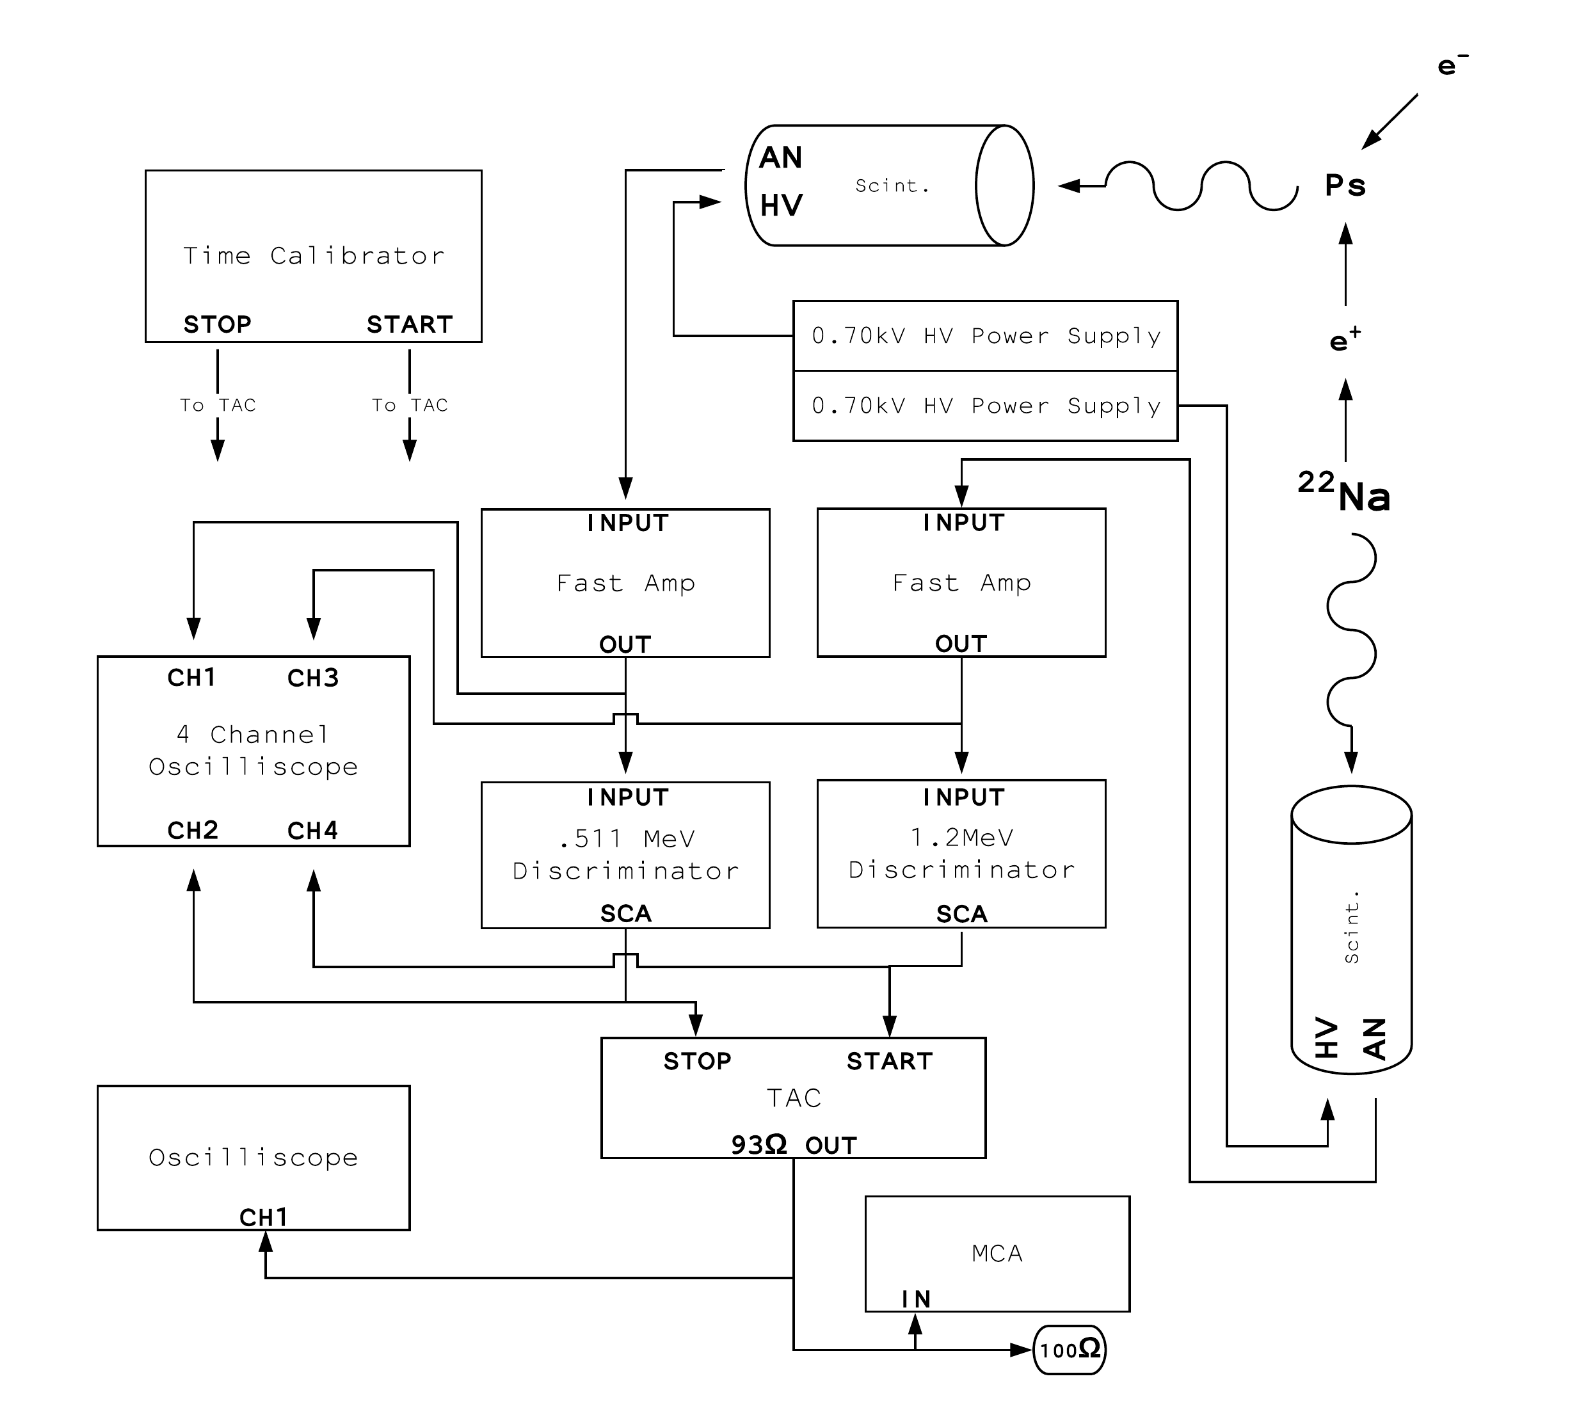
\includegraphics[width=4.5in]{apparatus.png}
        \caption{Apparatus connection diagram, taken from Zute, Campbell 2018}
    \end{center}
\end{figure}
Figure two shows the connection diagram for the apparatus, using BNC lines to connect various parts of the system.
\subsection{Scintillators}
A major portion of the detection is 2 NaI scintillators. These scintillators detect gamma rays and convert them into 
visible light, which is then amplified by a PMT (photomultiplier tube).
\subsection{TAC}
Another part is the Time-to-Amplitude Converter. This device produces a digital pulse for each analog pulse it senses above a set potential \cite{Zute:2018}.
\begin{figure}[!htbp]
    \begin{center}
        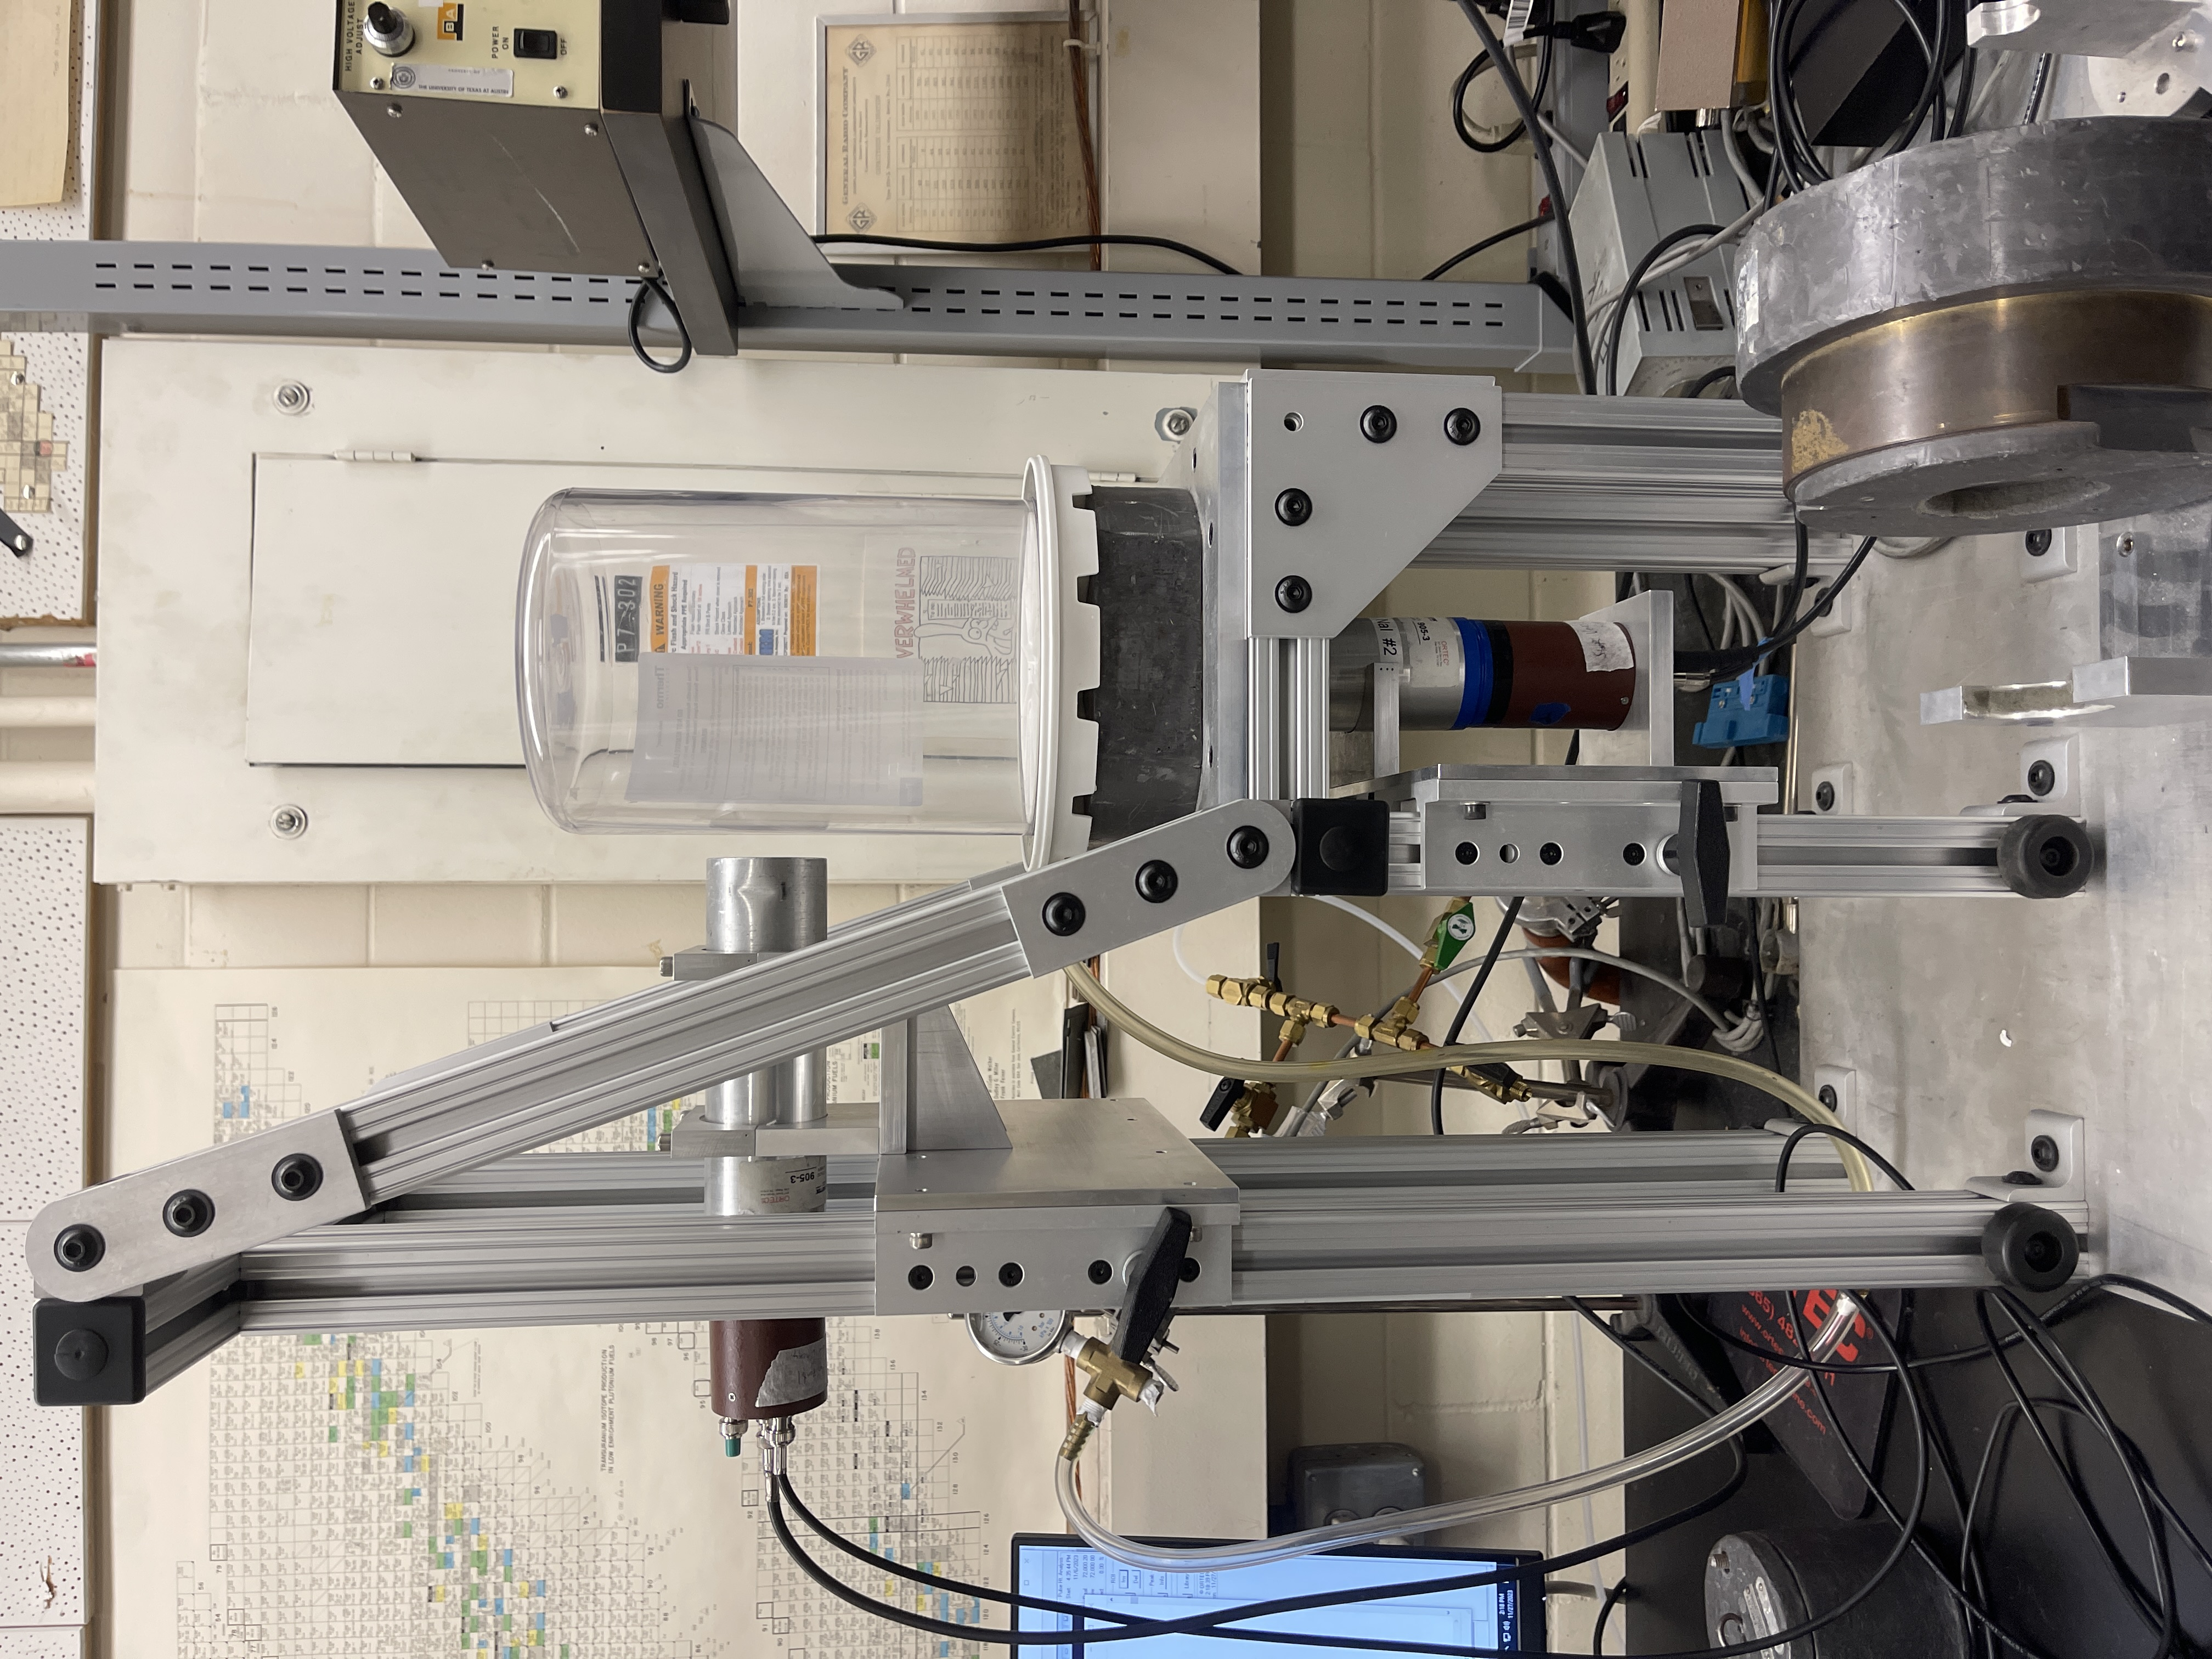
\includegraphics[width=5in, angle=270]{IMG_8886.JPG}
        \caption{Scintillator setup with orientations as described in Data Collection section}
    \end{center}
\end{figure}
\begin{figure}[!htbp]
    \begin{center}
        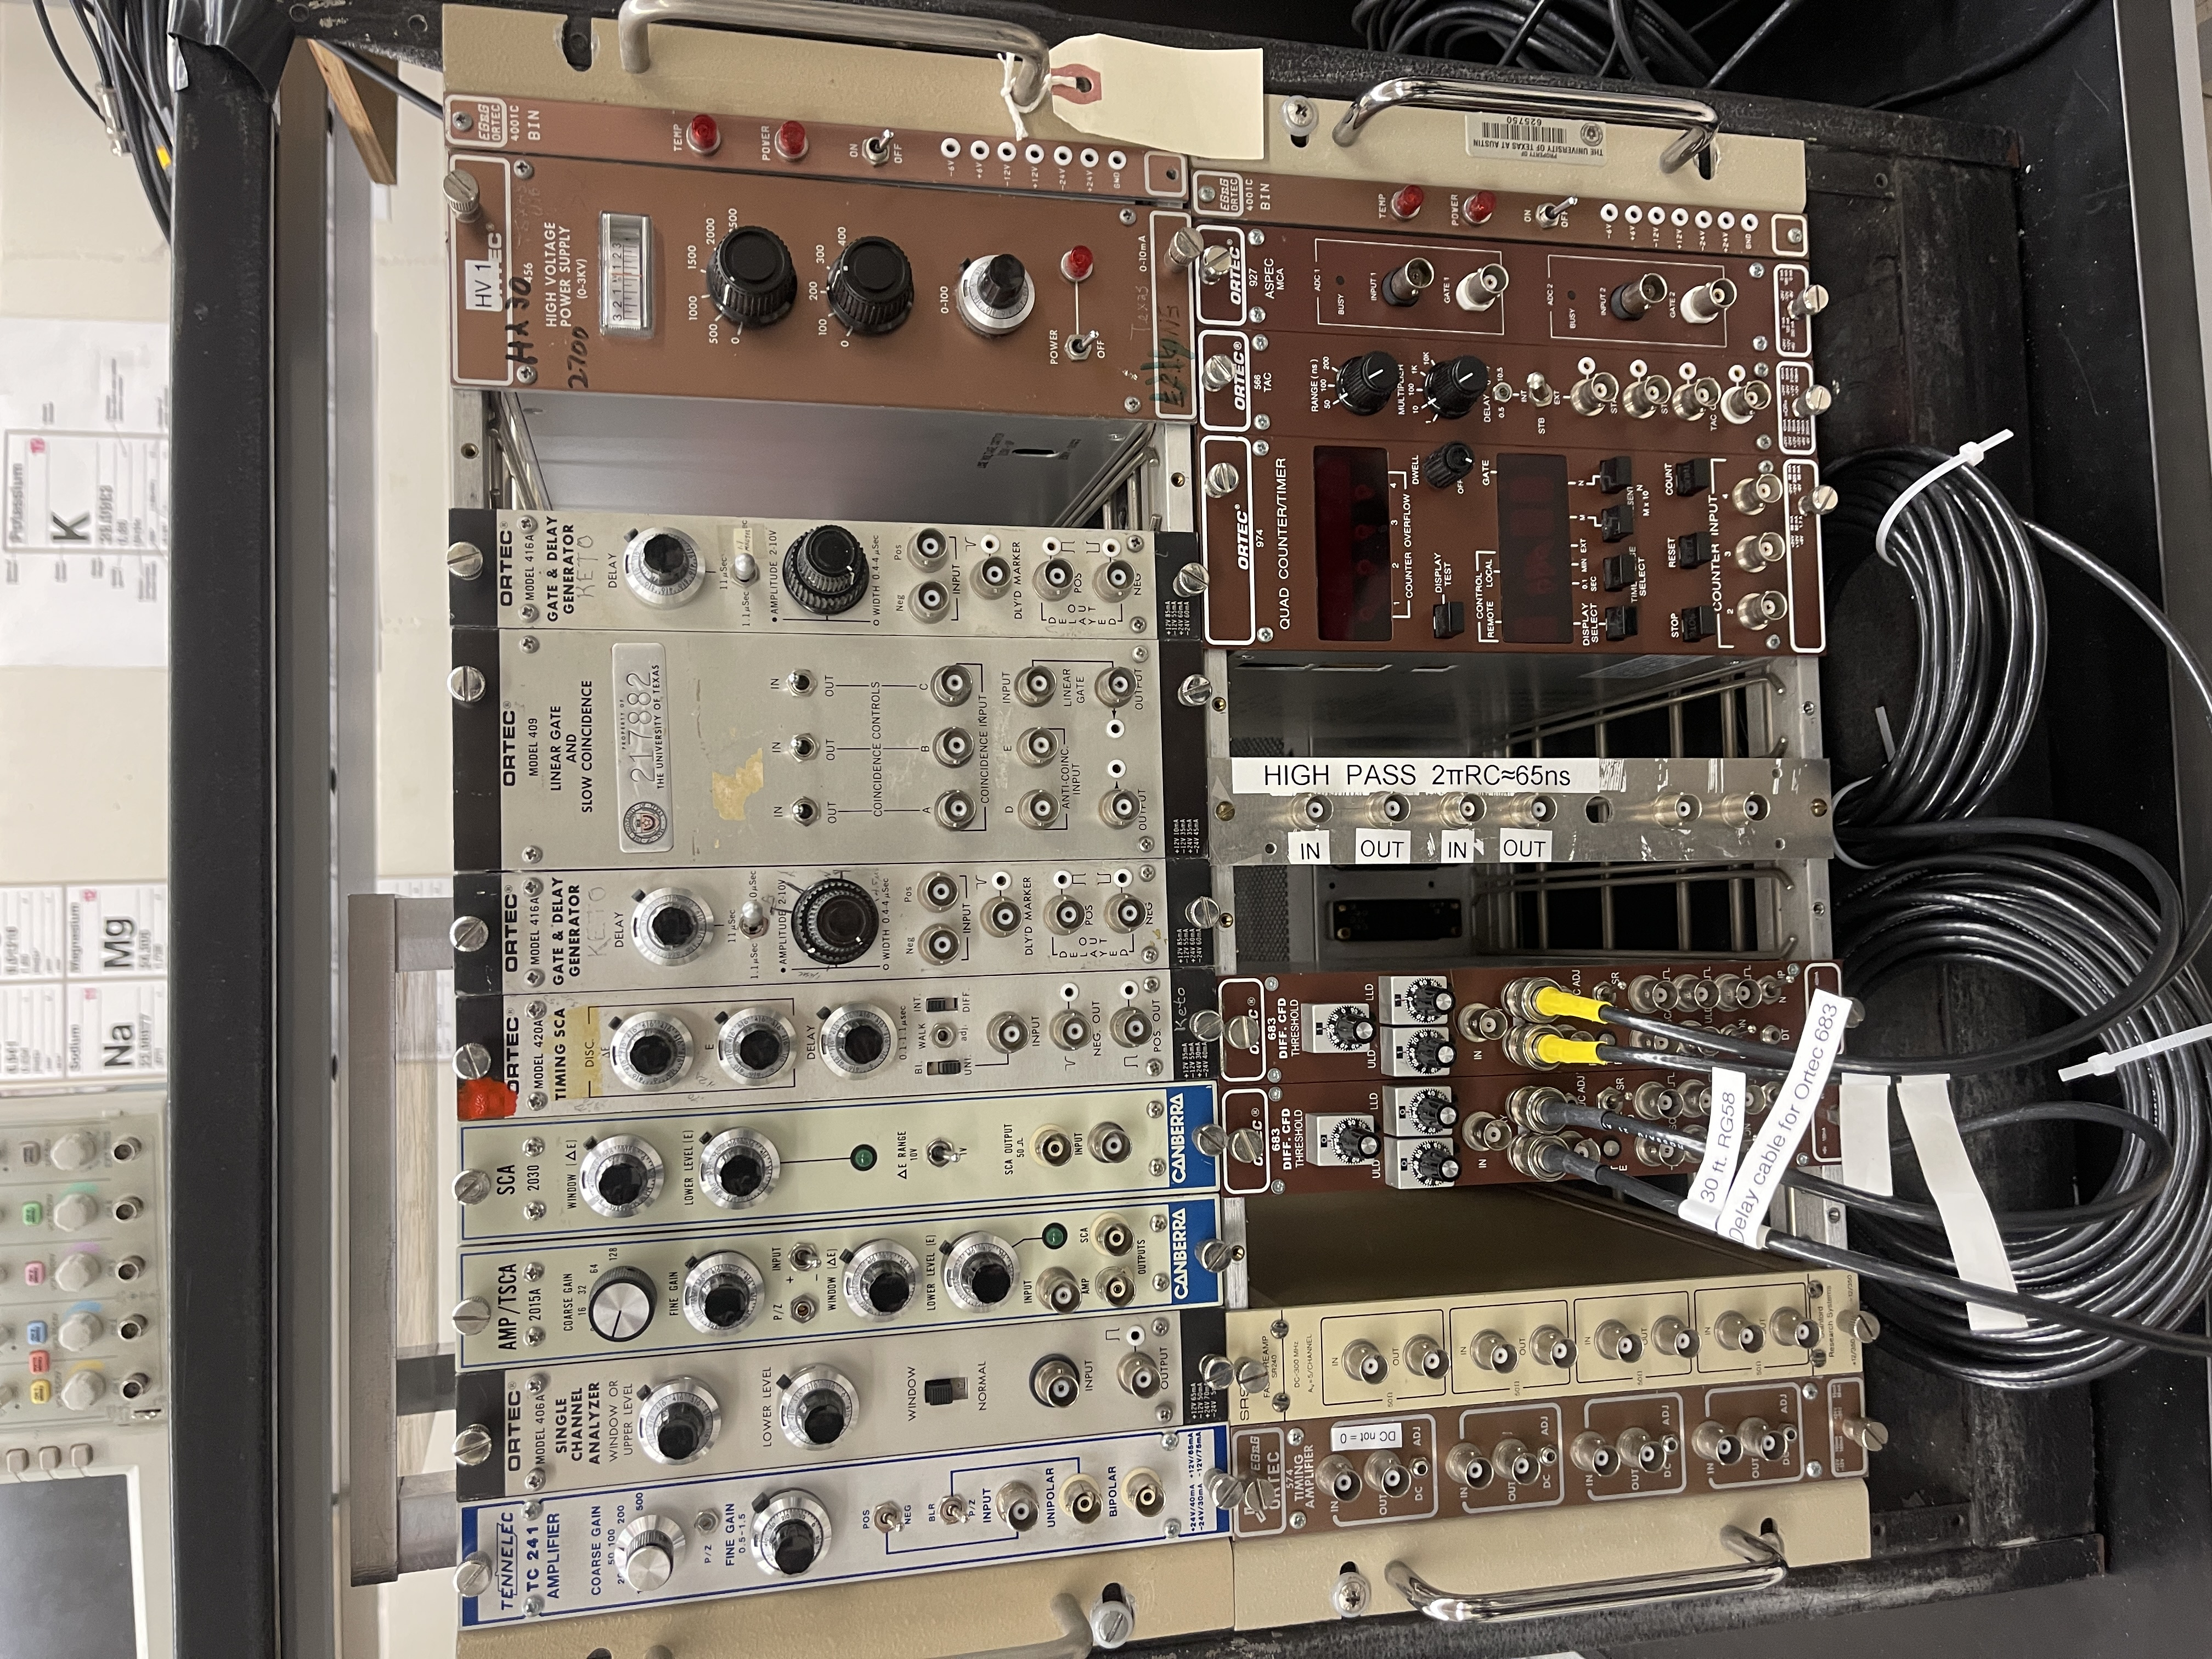
\includegraphics[width=5in, angle=270]{IMG_8887.JPG}
        \caption{ORTEC machines as descrived in Fig. 2}
    \end{center}
\end{figure}

\subsection{Data Collection}
The data collection process was long and very difficult to calibrate. First, we put the sample of Sodium-22 inside of 
a nitrogen filled chamber with two scintillators orthogonal to one another surrounding it. 
Typically, one is below the chamber, and one is perpenticular to the chamber, with both pointing towards the chamber itself.
After placing the button source inside the chamber, we connected the apparatus as described above, 
and calibrated the Maestro software in order to properly estimate the bin sizing with the time intervals associated.
After this, we let Maestro run for 24 hours, and saved the resultant .Chn file for analysis.
\section{Data Analysis}
Although we ran four trials for our data, we only found one viable run that gave us significant results. The flaws
in the other runs will be discussed below, but for now we will discuss the run we completed on November 15, 2023.
\begin{figure}[!htbp]
    \begin{center}
        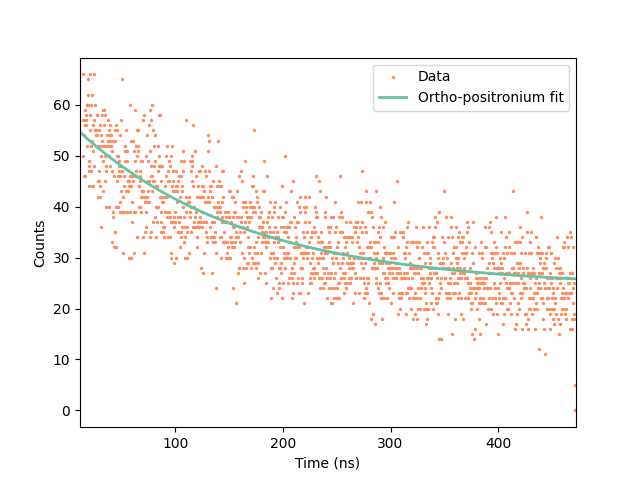
\includegraphics[width=4in, angle=0]{Figure_4.png}
        \caption{A plot showing the decay of the ortho-positronium. The plot should exhibit exponential decay, as explained in the aforementioned theory section.}
    \end{center}
\end{figure}
Our original data included thousands of counts for para-positronium data, however these were excluded as we were not measuring the half life of the para-positronium. 
Also, these counts were at such low time intervals that their accuracy cannot be determined to a sufficient degree of accuracy.

Fig. 5 generates a fit describing the activity of the sample with respect to time. The half life this line generates is 108.4 $\pm$ 7.7 ns.


\section{Summary and Conclusions}
First, let us discuss the reason our first three trials failed. some possible explanations for this failure can be attributed to background radiation, or an incorrect SCA calibration. 
In fact, the reason the first three trials were invalid was due to the fact that they all exhibited too many or too few counts. This leads us to believe that our SCA or TAC was calibrated in such a way
that led to too many or too few counts in Maestro.

Finally, our result for the half-life of the ortho-positronium was 108.4 $\pm$ 7.7 ns. This is below the accepted value, which is around 142ns in a vaccuum. Some reasons for this might be that we cut off our data too early. 
If our data analyzed too many para-positronium counts, this can explain why our value was below the accepted value for the lifetime of the ortho positronium.
\paragraph*{Acknowledgments}
I would like to thank my lab partner, Sannidhya Desai for his assistance on data
collection. Furthermore, I'd like to thank Dr. Dan Heinzen,
Parth Dave, and Konner Feldman for their assistance throughout the measurement and 
set up processes.

\bibliographystyle{plain} % We choose the "plain" reference style
\bibliography{refs} % Entries are in the refs.bib file

\end{document}

